\documentclass{amsart}
\usepackage{graphicx,float}
\usepackage{amsmath,xfrac,amssymb}
\usepackage{physics}
\usepackage{tikz}

 
\title{Quantum Field Theory Problem Sets}
\author{John Bortins}
 
\begin{document}
 
\maketitle{}
\begin{figure}[H]
    \centering
    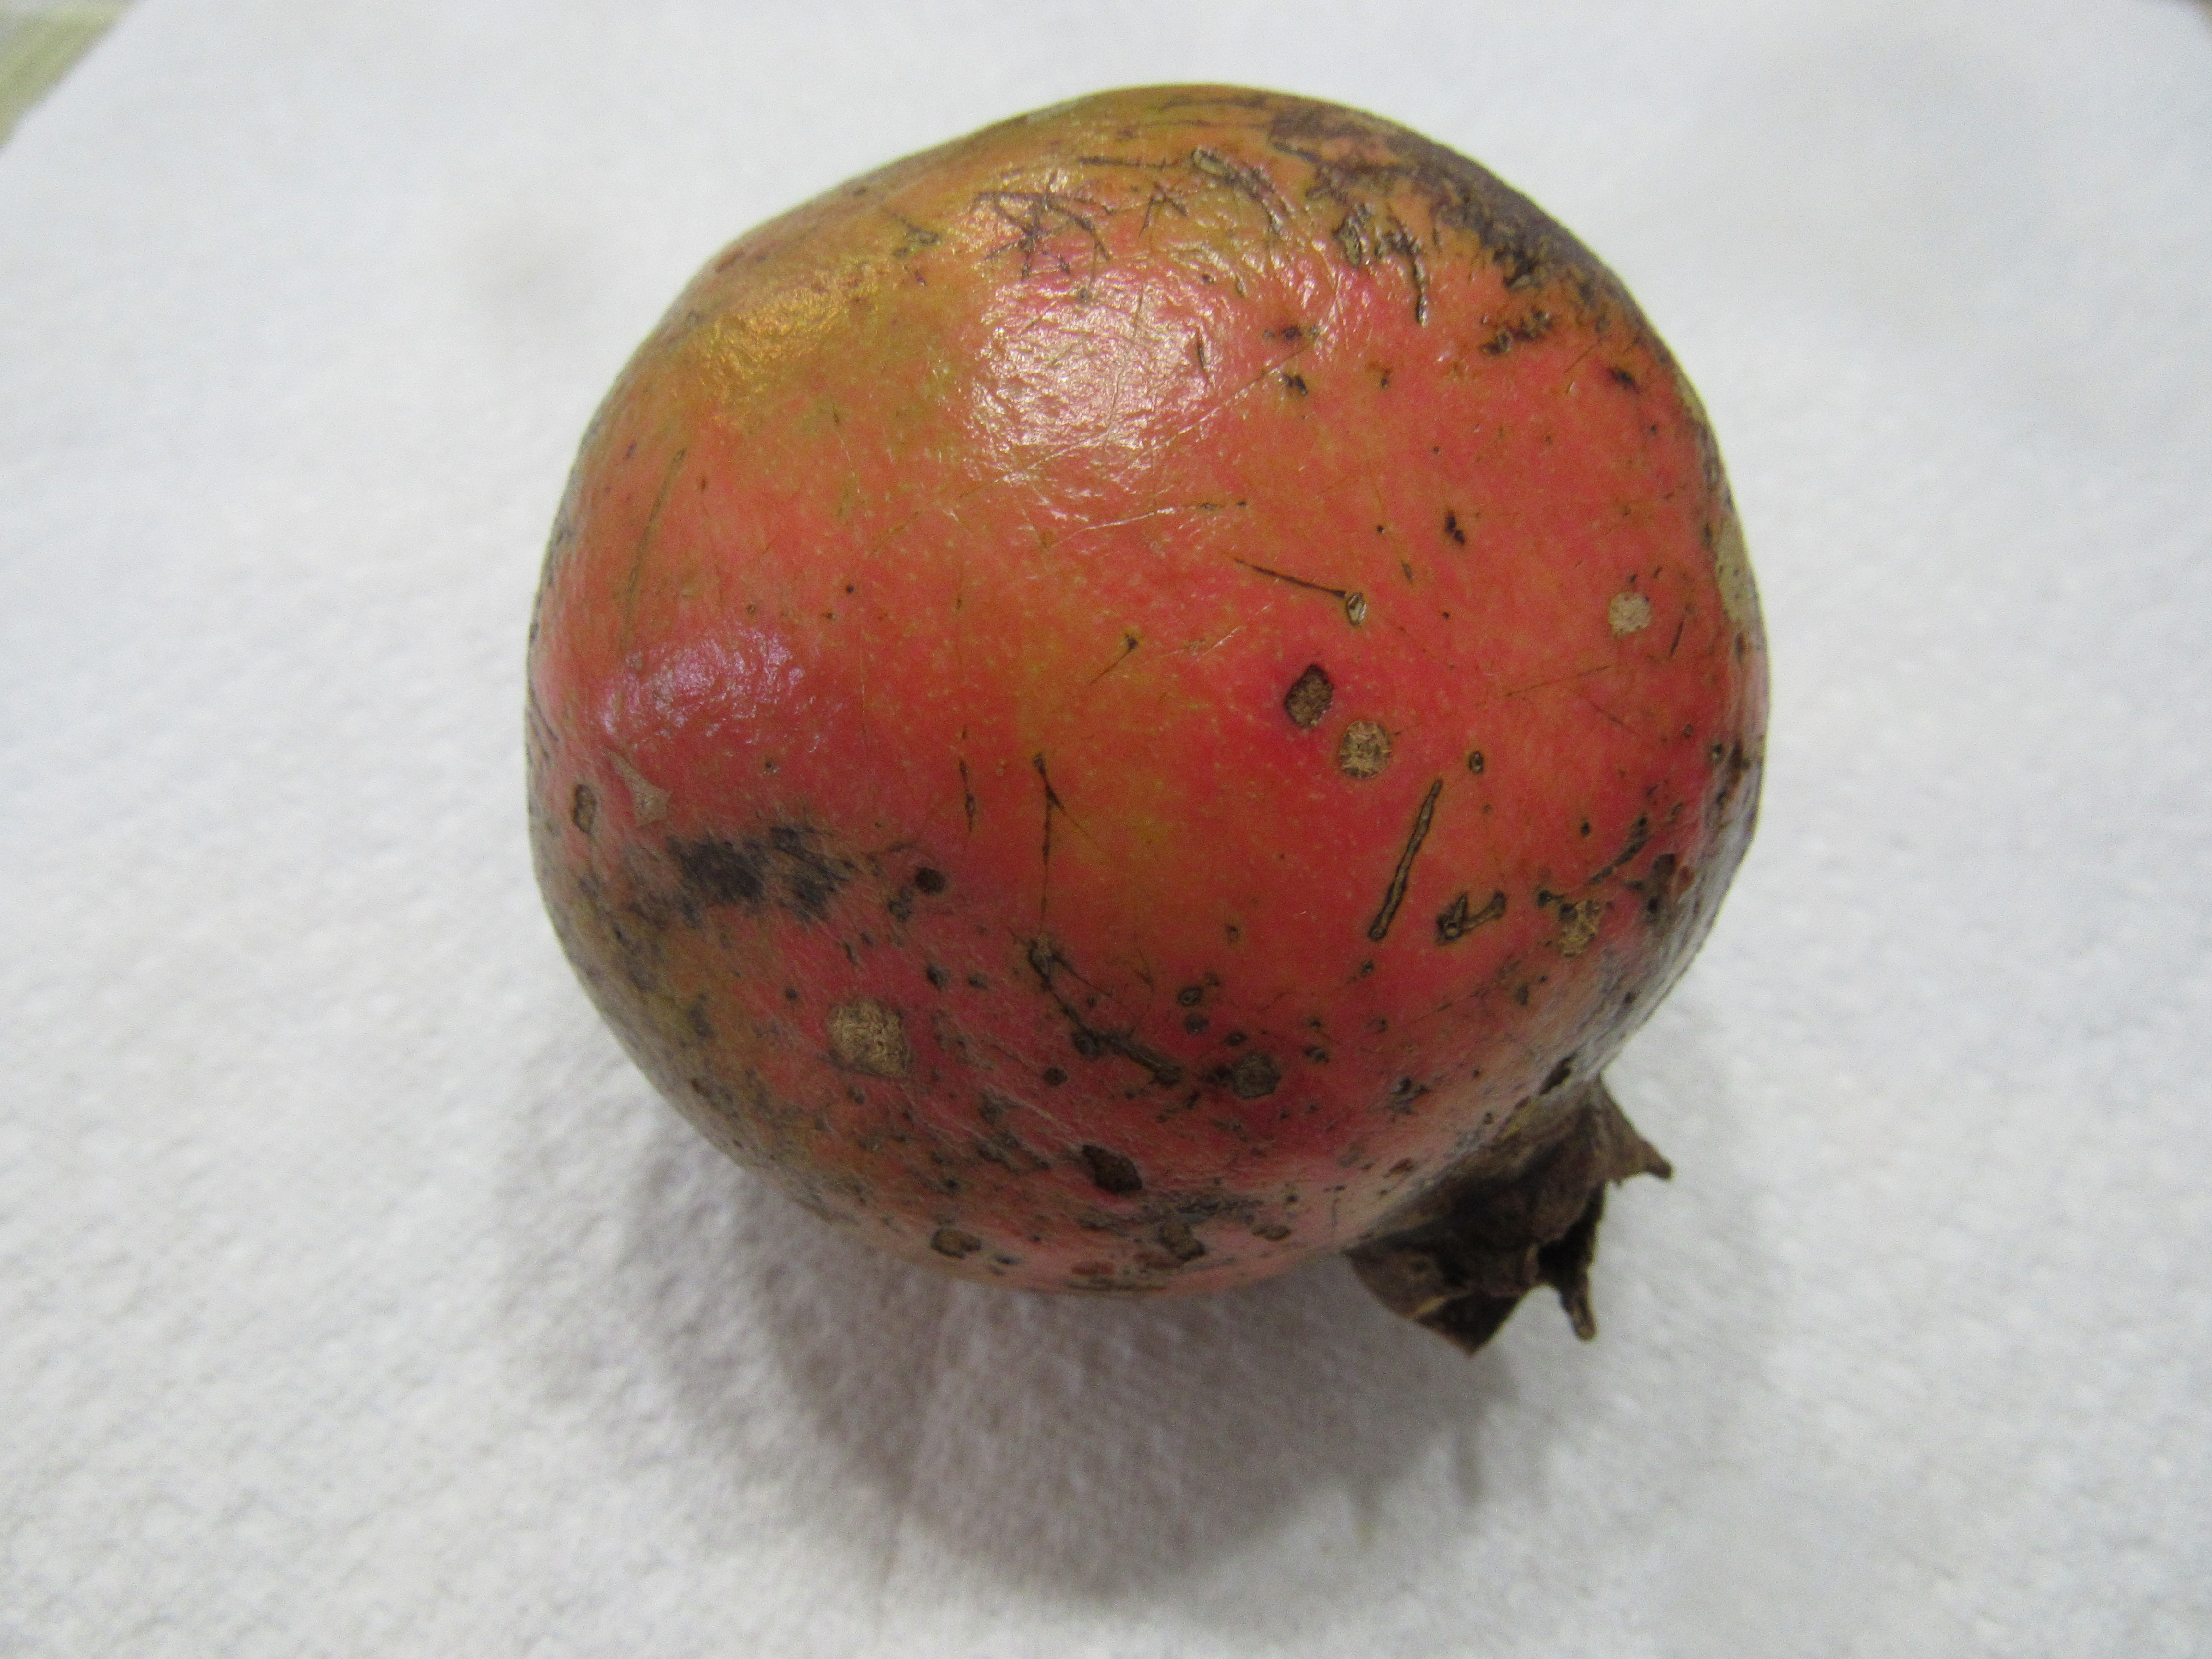
\includegraphics[width=0.5\textwidth]{IMG_0873}
    \caption{Pomegranate}
    \label{fig:awesome_image}
\end{figure}


\section*{Problem 3.1}

\[\text{For Boson operators satisfying}\qquad[\hat{a}_{\boldsymbol{p}},\hat{a}^\dagger_{\boldsymbol{q}}]  = \delta_{\boldsymbol{pq}}  \]

\[\text{Consider}\qquad \frac{1}{\mathcal{V}}\sum_{\boldsymbol{pq}}e^{i(\boldsymbol{p\cdot x}-\boldsymbol{q\cdot y})}[\hat{a}_{\boldsymbol{p}},\hat{a}^\dagger_{\boldsymbol{q}}]=\frac{1}{\mathcal{V}}\sum_{\boldsymbol{pq}}e^{i(\boldsymbol{p\cdot x}-\boldsymbol{q\cdot y})}\delta_{\boldsymbol{pq}}  \]
This picks off all cases where $\boldsymbol{p}=\boldsymbol{q}$ hence
\[\frac{1}{\mathcal{V}}\sum_{\boldsymbol{pq}}e^{i(\boldsymbol{p\cdot x}-\boldsymbol{q\cdot y})}[\hat{a}_{\boldsymbol{p}},\hat{a}^\dagger_{\boldsymbol{q}}]=\frac{1}{\mathcal{V}}\sum_{\boldsymbol{p}}e^{i\boldsymbol{p\cdot} (\boldsymbol{x}-\boldsymbol{y}) } \]
\[\text{Now}\qquad \boldsymbol{x}=\boldsymbol{y}\qq{implies} \frac{1}{\mathcal{V}}\sum_{\boldsymbol{p}}e^{i\boldsymbol{p\cdot} (\boldsymbol{x}-\boldsymbol{y})}=\frac{1}{\mathcal{V}}\sum_{\boldsymbol{p}}1=\frac{1}{\mathcal{V}}\mathcal{V}=1 \]

Where $\boldsymbol{x}\ne \boldsymbol{y}$ The sum catches all angles which must ultimately cancel each other giving a sum of zero.
\[\text{Therefore}\qquad\frac{1}{\mathcal{V}}\sum_{\boldsymbol{pq}}e^{i(\boldsymbol{p\cdot x}-\boldsymbol{q\cdot y})}[\hat{a}_{\boldsymbol{p}},\hat{a}^\dagger_{\boldsymbol{q}}]=\delta^{(3)} (\boldsymbol{x}-\boldsymbol{y})\qquad\blacksquare\]

\[\text{The same argument holds for Fermion operators satisfying}\qquad\{\hat{c}_{\boldsymbol{p}},\hat{c}^\dagger_{\boldsymbol{q}}\}  = \delta_{\boldsymbol{pq}}  \]
\[\text{Therefore}\qquad\frac{1}{\mathcal{V}}\sum_{\boldsymbol{pq}}e^{i(\boldsymbol{p\cdot x}-\boldsymbol{q\cdot y})}\{\hat{c}_{\boldsymbol{p}},\hat{c}^\dagger_{\boldsymbol{q}}\}=\delta^{(3)} (\boldsymbol{x}-\boldsymbol{y})\qquad\blacksquare\]

\section*{Problem 3.2}
Evaluate the following for the simple harmonic oscillator:
\[\text{(a)}\qquad[\hat{a},(\hat{a}^\dagger)^n]   \]
\[\text{Recall that}\qquad[\hat{a},\hat{a}^\dagger] = 1\qq{so for}n=1\qq{we do get}[\hat{a},(\hat{a}^\dagger)^1] =1(\hat{a}^\dagger)^0 \]

\[\text{Try the base case}\qquad n=2\qq{that is}[\hat{a},(\hat{a}^\dagger)^2] = \hat{a}(\hat{a}^\dagger)^2-(\hat{a}^\dagger)^2 \hat{a} = \hat{a}\hat{a}^\dagger \hat{a}^\dagger-\hat{a}^\dagger \hat{a}^\dagger \hat{a}   \]
\[[\hat{a},\hat{a}^\dagger] = 1 \implies \hat{a}\hat{a}^\dagger -1 =  \hat{a}^\dagger \hat{a}\]
\[\qq{which means}\hat{a}\hat{a}^\dagger \hat{a}^\dagger-\hat{a}^\dagger \hat{a}^\dagger \hat{a} =\hat{a}\hat{a}^\dagger \hat{a}^\dagger-\hat{a}^\dagger (\hat{a}\hat{a}^\dagger -1 ) =\hat{a}\hat{a}^\dagger \hat{a}^\dagger-\hat{a}^\dagger \hat{a}\hat{a}^\dagger +\hat{a}^\dagger\]
\[\qq{hence}\hat{a}\hat{a}^\dagger \hat{a}^\dagger-\hat{a}^\dagger \hat{a}\hat{a}^\dagger +\hat{a}^\dagger=(\hat{a}\hat{a}^\dagger -\hat{a}^\dagger \hat{a})\hat{a}^\dagger +\hat{a}^\dagger   =[\hat{a},\hat{a}^\dagger] \hat{a}^\dagger +\hat{a}^\dagger  = \hat{a}^\dagger +\hat{a}^\dagger \]
\[ [\hat{a},(\hat{a}^\dagger)^2]   =2\hat{a}^\dagger \]

\[\qq{Given the inductive step}[\hat{a},(\hat{a}^\dagger)^{n-1}] =(n-1)(\hat{a}^\dagger)^{n-2} \]
\[\qq{Try}[\hat{a},(\hat{a}^\dagger)^n]=\hat{a}(\hat{a}^\dagger)^n-(\hat{a}^\dagger)^n \hat{a}=\hat{a}(\hat{a}^\dagger)^{n-1}\hat{a}^\dagger-(\hat{a}^\dagger)^{n-1}\hat{a}^\dagger \hat{a}\]
\[=\hat{a}(\hat{a}^\dagger)^{n-1}\hat{a}^\dagger-(\hat{a}^\dagger)^{n-1}(\hat{a}\hat{a}^\dagger -1 )=\hat{a}(\hat{a}^\dagger)^{n-1}\hat{a}^\dagger-(\hat{a}^\dagger)^{n-1}\hat{a}\hat{a}^\dagger +(\hat{a}^\dagger)^{n-1}\]
\[=\hat{a}(\hat{a}^\dagger)^{n-1}\hat{a}^\dagger-(\hat{a}^\dagger)^{n-1}\hat{a}\hat{a}^\dagger +(\hat{a}^\dagger)^{n-1}=(\hat{a}(\hat{a}^\dagger)^{n-1}-(\hat{a}^\dagger)^{n-1}\hat{a})\hat{a}^\dagger +(\hat{a}^\dagger)^{n-1}\]
\[=[\hat{a},(\hat{a}^\dagger)^{n-1}]\hat{a}^\dagger +(\hat{a}^\dagger)^{n-1}=(n-1)(\hat{a}^\dagger)^{n-2}\hat{a}^\dagger+(\hat{a}^\dagger)^{n-1}=n(\hat{a}^\dagger)^{n-1}\]
\[\qq{Therefore}[\hat{a},(\hat{a}^\dagger)^n]=n(\hat{a}^\dagger)^{n-1}\qquad\blacksquare\]

\[\text{(b)}\qquad\bra{0}\hat{a}^n(\hat{a}^\dagger)^m\ket{0}   \]
\[\qq{Recall} \ket{k}=\frac{(\hat{a}^\dagger)^k}{\sqrt{k!}}\ket{0}\qq{hence} \ket{m}=\frac{(\hat{a}^\dagger)^m}{\sqrt{m!}}\ket{0} \qq{and}\ket{n}=\frac{(\hat{a}^\dagger)^n}{\sqrt{n!}}\ket{0}\]
\[\bra{0}\hat{a}^n(\hat{a}^\dagger)^m\ket{0} =\bra{n}\sqrt{n!}\sqrt{m!}\ket{m}=\sqrt{n!}\sqrt{m!}\bra{n}\ket{m}=\sqrt{n!}\sqrt{m!}\delta_{nm}=n!\delta_{n,m}\]
\[\qq{Therefore}\bra{0}\hat{a}^n(\hat{a}^\dagger)^m\ket{0} =n!\delta_{n,m}\qquad\blacksquare\]

\[\text{(c)}\qquad\bra{m}\hat{a}^\dagger\ket{n}   \]
\[\qq{Recall}\hat{a}^\dagger\ket{k}=\sqrt{k+1}\ket{k+1}\]
\[\bra{m}\hat{a}^\dagger\ket{n} = \bra{m}\sqrt{n+1}\ket{n+1}  = \sqrt{n+1}\bra{m}\ket{n+1}=\sqrt{n+1}\delta_{m,n+1}\]
\[\qq{Therefore}\bra{m}\hat{a}^\dagger\ket{n}  =\sqrt{n+1}\delta_{m,n+1}\qquad\blacksquare\]

\[\text{(d)}\qquad\bra{m}\hat{a}\ket{n}   \]
\[\qq{Recall}\hat{a}\ket{k}=\sqrt{k}\ket{k-1}\]
\[\bra{m}\hat{a}\ket{n} = \bra{m}\sqrt{n}\ket{n-1}  = \sqrt{n}\bra{m}\ket{n-1}=\sqrt{n}\delta_{m,n-1}\]
\[\qq{Therefore}\bra{m}\hat{a}\ket{n}  =\sqrt{n}\delta_{m,n-1}\qquad\blacksquare\]

\section*{Problem 3.3}
\[\qq{Let}\hat{H}=\frac{1}{2m}(\hat{p}^2_1+\hat{p}^2_2+\hat{p}^2_3) + \frac{1}{2}m\omega^2(\hat{x}^2_1+\hat{x}^2_2+\hat{x}^2_3) \]
\[\qq{Construct}\hat{a}_i=\sqrt{\frac{m\omega}{2\hbar}}\left(\hat{x}_i+\frac{i}{m\omega}\hat{p}_i\right)\qq{and}\hat{a}^\dagger_i=\sqrt{\frac{m\omega}{2\hbar}}\left(\hat{x}_i-\frac{i}{m\omega}\hat{p}_i\right)\qq{where}i\in\{1,2,3\}\]
\[[\hat{a}_i,\hat{a}^\dagger_j]=\frac{m\omega}{2\hbar}\left(\hat{x}_i+\frac{i}{m\omega}\hat{p}_i\right)\left(\hat{x}_j-\frac{i}{m\omega}\hat{p}_j\right)-\frac{m\omega}{2\hbar}\left(\hat{x}_j-\frac{i}{m\omega}\hat{p}_j\right)\left(\hat{x}_i+\frac{i}{m\omega}\hat{p}_i\right)\]
\[[\hat{a}_i,\hat{a}^\dagger_j]=\frac{m\omega}{2\hbar}\left(\hat{x}_i\hat{x}_j-\hat{x}_j\hat{x}_i\right)+\frac{i}{2\hbar}\left(-\hat{x}_i\hat{p}_j+\hat{p}_i\hat{x}_j-\hat{x}_j\hat{p}_i+\hat{p}_j\hat{x}_i\right)+\frac{1}{2\hbar m\omega}\left(\hat{p}_i\hat{p}_j-\hat{p}_j\hat{p}_i\right)\]
\[[\hat{a}_i,\hat{a}^\dagger_j]=\frac{m\omega}{2\hbar}\left(\hat{x}_i\hat{x}_j-\hat{x}_j\hat{x}_i\right)+\frac{i}{2\hbar}\left(-[\hat{x}_i,\hat{p}_j]+[\hat{p}_i,\hat{x}_j]\right)+\frac{1}{2\hbar m\omega}\left(\hat{p}_i\hat{p}_j-\hat{p}_j\hat{p}_i\right)\]
The $\hat{x}_i,\hat{x}_j$ commute. The $\hat{p}_i,\hat{p}_j$ commute.
\[\qq{Hence}[\hat{a}_i,\hat{a}^\dagger_j]=\frac{i}{2\hbar}\left(-[\hat{x}_i,\hat{p}_j]+[\hat{p}_i,\hat{x}_j]\right)=\frac{i}{2\hbar}\left(-i\hbar\delta_{i,j}-i\hbar\delta_{i,j}\right)\]
\[\qq{So}[\hat{a}_i,\hat{a}^\dagger_j]=\delta_{i,j}\qq{where}i,j\in\{1,2,3\}\qquad\blacksquare\]

\[\qq{Now}\hat{a}^\dagger_i\hat{a}_i=\frac{m\omega}{2\hbar}\left(\hat{x}_i-\frac{i}{m\omega}\hat{p}_i\right)\left(\hat{x}_i+\frac{i}{m\omega}\hat{p}_i\right)=\frac{m\omega}{2\hbar}\left(\hat{x}^2_i+\frac{i}{m\omega}\hat{x}_i\hat{p}_i-\frac{i}{m\omega}\hat{p}_i\hat{x}_i+\frac{1}{m^2\omega^2}\hat{p}^2_i\right)\]


\[\hbar\omega\hat{a}^\dagger_i\hat{a}_i=\frac{m\omega^2}{2}\left(\hat{x}^2_i+\frac{i}{m\omega}[\hat{x}_i,\hat{p}_i]+\frac{1}{m^2\omega^2}\hat{p}^2_i\right)=\frac{1}{2m}\hat{p}^2_i+\frac{1}{2}m\omega^2\hat{x}^2_i+\frac{m\omega^2}{2}\frac{i}{m\omega}i\hbar\]
\[\hbar\omega\hat{a}^\dagger_i\hat{a}_i+\frac{1}{2}\hbar\omega=\frac{1}{2m}\hat{p}^2_i+\frac{1}{2}m\omega^2\hat{x}^2_i\]
\[\hat{H}=\hbar\omega\sum_i\left(\hat{a}^\dagger_i\hat{a}_i+\frac{1}{2}\right)\qq{where}i\in\{1,2,3\}\qquad\blacksquare\]

\[\qq{Construct}\hat{b}^\dagger_1=-\frac{1}{\sqrt{2}}\left(\hat{a}^\dagger_1+i\hat{a}^\dagger_2\right)\qq{,}\hat{b}^\dagger_0=\hat{a}^\dagger_3\qq{and}\hat{b}_{-1}=\frac{1}{\sqrt{2}}\left(\hat{a}^\dagger_1-i\hat{a}^\dagger_2\right)\]
First demonstrate a lemma:
\begin{align*}
[A+B,C+D]&=(A+B)(C+D)-(C+D)(A+B)\\
&=AC+AD+BC+BD-CA-CB-DA-DB\\
&=AC-CA+AD-DA+BC-CB+BD-DB\\
[A+B,C+D]&=[A,C]+[A,D]+[B,C]+[B,D]\qquad\blacksquare
\end{align*}
\begin{align*}
[\hat{b}_0,\hat{b}^\dagger_0]&=[\hat{a}_3,\hat{a}^\dagger_3]=1\\
[\hat{b}_0,\hat{b}^\dagger_1]&=[\hat{a}_3,-\frac{1}{\sqrt{2}}\left(\hat{a}^\dagger_1+i\hat{a}^\dagger_2\right)]=-\frac{1}{\sqrt{2}}[\hat{a}_3,\hat{a}^\dagger_1]-\frac{i}{\sqrt{2}}[\hat{a}_3,\hat{a}^\dagger_2]=0\\
[\hat{b}_0,\hat{b}^\dagger_{-1}]&=[\hat{a}_3,\frac{1}{\sqrt{2}}\left(\hat{a}^\dagger_1-i\hat{a}^\dagger_2\right)]=\frac{1}{\sqrt{2}}[\hat{a}_3,\hat{a}^\dagger_1]-\frac{i}{\sqrt{2}}[\hat{a}_3,\hat{a}^\dagger_2]=0\\
[\hat{b}_1,\hat{b}^\dagger_0]&=[-\frac{1}{\sqrt{2}}\left(\hat{a}_1-i\hat{a}_2\right),\hat{a}^\dagger_3]=-\frac{1}{\sqrt{2}}[\hat{a}_1,\hat{a}^\dagger_3]-\frac{i}{\sqrt{2}}[\hat{a}_2,\hat{a}^\dagger_3]=0\\
[\hat{b}_1,\hat{b}^\dagger_1]&=[-\frac{1}{\sqrt{2}}\left(\hat{a}_1-i\hat{a}_2\right),-\frac{1}{\sqrt{2}}\left(\hat{a}^\dagger_1+i\hat{a}^\dagger_2\right)]=\frac{1}{2}[\hat{a}_1,\hat{a}^\dagger_1]+\frac{i}{2}[\hat{a}_1,\hat{a}^\dagger_2]+\frac{-i}{2}[\hat{a}_2,\hat{a}^\dagger_1]+\frac{1}{2}[\hat{a}_2,\hat{a}^\dagger_2]=1\\
[\hat{b}_1,\hat{b}^\dagger_{-1}]&=[-\frac{1}{\sqrt{2}}\left(\hat{a}_1-i\hat{a}_2\right),\frac{1}{\sqrt{2}}\left(\hat{a}^\dagger_1-i\hat{a}^\dagger_2\right)]=-\frac{1}{2}[\hat{a}_1,\hat{a}^\dagger_1]-\frac{-i}{2}[\hat{a}_1,\hat{a}^\dagger_2]-\frac{-i}{2}[\hat{a}_2,\hat{a}^\dagger_1]-\frac{-1}{2}[\hat{a}_2,\hat{a}^\dagger_2]=0\\
[\hat{b}_{-1},\hat{b}^\dagger_0]&=[\frac{1}{\sqrt{2}}\left(\hat{a}_1+i\hat{a}_2\right),\hat{a}^\dagger_3]=\frac{1}{\sqrt{2}}[\hat{a}_1,\hat{a}^\dagger_3]-\frac{i}{\sqrt{2}}[\hat{a}_2,\hat{a}^\dagger_3]=0\\
[\hat{b}_{-1},\hat{b}^\dagger_1]&=[\frac{1}{\sqrt{2}}\left(\hat{a}_1+i\hat{a}_2\right),-\frac{1}{\sqrt{2}}\left(\hat{a}^\dagger_1+i\hat{a}^\dagger_2\right)]=-\frac{1}{2}[\hat{a}_1,\hat{a}^\dagger_1]-\frac{i}{2}[\hat{a}_1,\hat{a}^\dagger_2]-\frac{i}{2}[\hat{a}_2,\hat{a}^\dagger_1]-\frac{-1}{2}[\hat{a}_2,\hat{a}^\dagger_2]=0\\
[\hat{b}_{-1},\hat{b}^\dagger_{-1}]&=[\frac{1}{\sqrt{2}}\left(\hat{a}_1+i\hat{a}_2\right),\frac{1}{\sqrt{2}}\left(\hat{a}^\dagger_1-i\hat{a}^\dagger_2\right)]=\frac{1}{2}[\hat{a}_1,\hat{a}^\dagger_1]+\frac{-i}{2}[\hat{a}_1,\hat{a}^\dagger_2]+\frac{i}{2}[\hat{a}_2,\hat{a}^\dagger_1]+\frac{1}{2}[\hat{a}_2,\hat{a}^\dagger_2]=1
\end{align*}
\[\qq{Therefore}[\hat{b}_{i},\hat{b}^\dagger_{j}]=\delta_{i,j}\qq{where}i,j\in\{-1,0,1\}\qquad\blacksquare\]

\[\qq{Construct}\hat{b}^\dagger_i\hat{b}_i\qq{where}i\in\{-1,0,1\}\]
\begin{align*}
\hat{b}^\dagger_{-1}\hat{b}_{-1}&=\frac{1}{2}\left(\hat{a}^\dagger_1+i\hat{a}^\dagger_2\right)\left(\hat{a}_1-i\hat{a}_2\right)=\frac{1}{2}\left(\hat{a}^\dagger_1\hat{a}_1-i\hat{a}^\dagger_1\hat{a}_2+i\hat{a}^\dagger_2\hat{a}_1+\hat{a}^\dagger_2\hat{a}_2\right)\\
\hat{b}^\dagger_0\hat{b}_0&=\hat{a}^\dagger_3\hat{a}_3\\
\hat{b}^\dagger_1\hat{b}_1&=\hat{b}_{-1}=\frac{1}{2}\left(\hat{a}^\dagger_1-i\hat{a}^\dagger_2\right)\left(\hat{a}_1+i\hat{a}_2\right)=\frac{1}{2}\left(\hat{a}^\dagger_1\hat{a}_1+i\hat{a}^\dagger_1\hat{a}_2-i\hat{a}^\dagger_2\hat{a}_1+\hat{a}^\dagger_2\hat{a}_2\right)
\end{align*}
\[\qq{Clearly}\sum_i \hat{b}^\dagger_{i}\hat{b}_{i}=\sum_j \hat{a}^\dagger_{j}\hat{a}_{j}\qq{where}i\in\{-1,0,1\}\qq{where}j\in\{1,2,3\}\]
\[\qq{Hence}\hat{H}=\hbar\omega\sum_i\left(\hat{b}^\dagger_i\hat{b}_i+\frac{1}{2}\right)\qq{where}i\in\{-1,0,1\}\qquad\blacksquare\]

\[\qq{Define}\hat{L}^i=-i\hbar \epsilon^{ijk}\hat{a}^\dagger_j\hat{a}_k\qq{e.g.,}\hat{L}^3=-i\hbar\left(\epsilon^{312}\hat{a}^\dagger_1\hat{a}_2 +\epsilon^{321}\hat{a}^\dagger_2\hat{a}_1\right)=-i\hbar\left(\hat{a}^\dagger_1\hat{a}_2 -\hat{a}^\dagger_2\hat{a}_1\right)\]
\[\qq{Examine}\hat{b}^\dagger_1+\hat{b}^\dagger_{-1}=-\frac{2i}{\sqrt{2}}\hat{a}^\dagger_2 \qq{and}\hat{b}^\dagger_1-\hat{b}^\dagger_{-1}=-\frac{2}{\sqrt{2}}\hat{a}^\dagger_1    \]
\[\qq{Therefore}\hat{a}^\dagger_2=\frac{i\sqrt{2}}{2}\left(\hat{b}^\dagger_1+\hat{b}^\dagger_{-1}\right) \qq{and}\hat{a}^\dagger_1=-\frac{\sqrt{2}}{2}\left(\hat{b}^\dagger_1-\hat{b}^\dagger_{-1} \right)   \]
\begin{align*}
\hat{a}^\dagger_1\hat{a}_2 -\hat{a}^\dagger_2\hat{a}_1&=-\frac{i}{2}\left(\hat{b}^\dagger_1-\hat{b}^\dagger_{-1} \right)\left(\hat{b}_1+\hat{b}_{-1}\right)-\frac{i}{2}\left(\hat{b}^\dagger_1+\hat{b}^\dagger_{-1}\right)\left(\hat{b}_1-\hat{b}_{-1}\right)\\
&=-\frac{i}{2}\hat{b}^\dagger_1 \hat{b}_1-\frac{i}{2}\hat{b}^\dagger_1 \hat{b}_{-1}+\frac{i}{2}\hat{b}^\dagger_{-1} \hat{b}_1+\frac{i}{2}\hat{b}^\dagger_{-1} \hat{b}_{-1}-\frac{i}{2}\hat{b}^\dagger_1 \hat{b}_1+\frac{i}{2}\hat{b}^\dagger_1 \hat{b}_{-1}-\frac{i}{2}\hat{b}^\dagger_{-1} \hat{b}_1+\frac{i}{2}\hat{b}^\dagger_{-1} \hat{b}_{-1}\\
&=-i\hat{b}^\dagger_1 \hat{b}_1+i\hat{b}^\dagger_{-1} \hat{b}_{-1}
\end{align*}
\[\hat{L}^3=\hbar\hat{b}^\dagger_1 \hat{b}_1-\hbar\hat{b}^\dagger_{-1} \hat{b}_{-1}=\hbar\sum_m m\hat{b}^\dagger_m \hat{b}_m\qq{where}m\in\{-1,0,1\}\qquad\blacksquare\]


\section*{Problem 3.4}
\[\qq{For fermions}\hat{c}^\dagger_1 \hat{c}^\dagger_2\ket{0}=-\hat{c}^\dagger_2 \hat{c}^\dagger_1\ket{0}  \]

Consider the determinants
\[
\begin{vmatrix} a & b \\ c & d \end{vmatrix}=ad-bc\qq{,} \begin{vmatrix} b & a \\ d & c \end{vmatrix}=bc-da\qq{,} \begin{vmatrix} c & d \\ a & b \end{vmatrix}=cb-ad.
\]
Interchanging columns or rows gets back the negative of the original determinant.

Express the wave functions using a determinant
\[
\begin{vmatrix} \psi_1(r_1) & \psi_2(r_1) \\ \psi_1(r_2) & \psi_2(r_2) \end{vmatrix}=\psi_1(r_1) \psi_2(r_2) -\psi_1(r_2) \psi_2(r_1).
\]
Then swap columns
\[
\begin{vmatrix}  \psi_2(r_1) & \psi_1(r_1)\\  \psi_2(r_2) & \psi_1(r_2)\end{vmatrix}= \psi_2(r_1)\psi_1(r_2)-\psi_2(r_2)\psi_1(r_1)=-[ \psi_2(r_2)\psi_1(r_1) - \psi_2(r_1)\psi_1(r_2)].
\]
Normalize and wave hands vigorously to extend the idea to $N$.


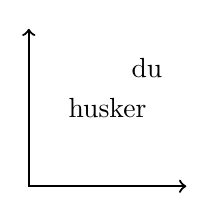
\begin{tikzpicture}
\draw [thick, <->] (0,2) -- (0,0) -- (2,0);
\node at (1,1) {husker};
\node at (3/2,3/2) {du};
\end{tikzpicture}

\end{document}
